\documentclass[12pt,a4paper,]{harvard-thesis}


\usepackage{layouts}

% Overwrite \begin{figure}[htbp] with \begin{figure}[H]
\usepackage{float}
\let\origfigure\figure
\let\endorigfigure\endfigure
\renewenvironment{figure}[1][2] {
    \expandafter\origfigure\expandafter[H]
} {
    \endorigfigure
}


% fix for pandoc 1.14
\providecommand{\tightlist}{%
  \setlength{\itemsep}{0pt}\setlength{\parskip}{0pt}}

% TP: hack to truncate list of figures/tables.
\usepackage{truncate}
\usepackage{caption}
\usepackage{tocloft}
% TP: end hack

\usepackage{amssymb,amsmath}
\usepackage{ifxetex,ifluatex}
\ifnum 0\ifxetex 1\fi\ifluatex 1\fi=0 % if pdftex
  \usepackage[T1]{fontenc}
  \usepackage[utf8]{inputenc}
\else % if luatex or xelatex
  \ifxetex
    \usepackage{mathspec}
    \usepackage{xltxtra,xunicode}
  \else
    \usepackage{fontspec}
  \fi
  \defaultfontfeatures{Mapping=tex-text,Scale=MatchLowercase}
  \newcommand{\euro}{€}
\fi
% use upquote if available, for straight quotes in verbatim environments
\IfFileExists{upquote.sty}{\usepackage{upquote}}{}
% use microtype if available
\IfFileExists{microtype.sty}{%
\usepackage{microtype}
\UseMicrotypeSet[protrusion]{basicmath} % disable protrusion for tt fonts
}{}
\usepackage{graphicx}
\makeatletter
\def\maxwidth{\ifdim\Gin@nat@width>\linewidth\linewidth\else\Gin@nat@width\fi}
\def\maxheight{\ifdim\Gin@nat@height>\textheight\textheight\else\Gin@nat@height\fi}
\makeatother
% Scale images if necessary, so that they will not overflow the page
% margins by default, and it is still possible to overwrite the defaults
% using explicit options in \includegraphics[width, height, ...]{}
\setkeys{Gin}{width=\maxwidth,height=\maxheight,keepaspectratio}

\setlength{\parindent}{0pt}
\setlength{\parskip}{6pt plus 2pt minus 1pt}
\setlength{\emergencystretch}{3em}  % prevent overfull lines
\setcounter{secnumdepth}{5}

\date{}
\makeatletter
\@ifpackageloaded{subfig}{}{\usepackage{subfig}}
\@ifpackageloaded{caption}{}{\usepackage{caption}}
\captionsetup[subfloat]{margin=0.5em}
\AtBeginDocument{%
\renewcommand*\figurename{Figure}
\renewcommand*\tablename{Table}
}
\AtBeginDocument{%
\renewcommand*\listfigurename{List of Figures}
\renewcommand*\listtablename{List of Tables}
}
\@ifpackageloaded{float}{}{\usepackage{float}}
\floatstyle{ruled}
\@ifundefined{c@chapter}{\newfloat{codelisting}{h}{lop}}{\newfloat{codelisting}{h}{lop}[chapter]}
\floatname{codelisting}{Listing}
\newcommand*\listoflistings{\listof{codelisting}{List of Listings}}
\makeatother

\begin{document}

\begin{titlepage}
    \begin{center}

    % Delete the following line
    % to remove the UCL header logo
    %\ThisULCornerWallPaper{1.0}{style/univ_logo.eps}
        
        \vspace*{2.5cm}
        
        \huge
        The thing with the Golgi apparatus
        
        \vspace{1.5cm}
        
        \Large
        Gert-Jan Both

        \vspace{1.5cm}

        %\normalsize
        %A thesis presented for the degree of\\
        %Doctor of Philosophy
        
        \vfill
        
        \normalsize
        Supervised by:\\
        P. Sens\\
        C. Storm

        \vspace{0.8cm}

        % Uncomment the following line
        % to add a centered university logo
        % 
\includegraphics[width=0.4\textwidth]{style/univ_logo.eps}
        
        \normalsize
        Technical university of Eindhoven\\
        January-November 2018

        % Except where otherwise noted, content in this thesis is licensed under a Creative Commons Attribution 4.0 License (http://creativecommons.org/licenses/by/4.0), which permits unrestricted use, distribution, and reproduction in any medium, provided the original work is properly cited. Copyright 2015,Tom Pollard.

    \end{center}
\end{titlepage}

\hypertarget{abstract}{%
\chapter*{Abstract}\label{abstract}}
\addcontentsline{toc}{chapter}{Abstract}

Lorem ipsum dolor sit amet, consectetur adipiscing elit. Nam et turpis
gravida, lacinia ante sit amet, sollicitudin erat. Aliquam efficitur
vehicula leo sed condimentum. Phasellus lobortis eros vitae rutrum
egestas. Vestibulum ante ipsum primis in faucibus orci luctus et
ultrices posuere cubilia Curae; Donec at urna imperdiet, vulputate orci
eu, sollicitudin leo. Donec nec dui sagittis, malesuada erat eget,
vulputate tellus. Nam ullamcorper efficitur iaculis. Mauris eu vehicula
nibh. In lectus turpis, tempor at felis a, egestas fermentum massa.

\pagenumbering{roman}
\setcounter{page}{1}
\newpage
\pagenumbering{gobble}

\tableofcontents

\newpage

\hypertarget{introduction}{%
\chapter{Introduction}\label{introduction}}

\hypertarget{quantitative-work-on-the-golgi-so-far}{%
\section{Quantitative work on the Golgi so
far}\label{quantitative-work-on-the-golgi-so-far}}

\hypertarget{rush-system}{%
\section{RUSH system}\label{rush-system}}

\hypertarget{man-ii}{%
\subsection{Man II}\label{man-ii}}

\hypertarget{introduction-1}{%
\chapter{Introduction}\label{introduction-1}}

\hypertarget{data-processing-pipeline}{%
\chapter{Data processing pipeline}\label{data-processing-pipeline}}

In this chapter I present the work done on processing the rush movies.
Several preprocssing steps hav been undertaken to improve the quality of
the fit, and we present all here. Roughly, we can divide the process in
four steps:

\begin{enumerate}
\def\labelenumi{\arabic{enumi}.}
\tightlist
\item
  Segmentation and creation of masks
\item
  Denoising of movies
\item
  Calculation of spatial and temporal derivatives
\item
  The actual fitting
\end{enumerate}

Below we describe each step separately.

\hypertarget{step-1-segmentation}{%
\section{Step 1: Segmentation}\label{step-1-segmentation}}

The images obtained from the rush experiments often contain multiple
cells. Furthermore, we can also segment the image into roughly three
different types: 1) the background, where nothing of interest happens.
No cells are present here, 2) the cytoplasm, which is the area where we
want to fit our model and 3) the Golgi itself, where we do not
necessarily want to fit. Unfortunately, no bright field images were
available, making segmentation significantly harder, as no clear cell
boundary can be observed. Further complicating the story is the large
dynamic range of the movies due to the fluorescence concentrating in the
Golgi. The following procedures we present have been developed to deal
with these problems. Note that they are empirical methods, i.e.~there's
no theoretical background as to why they \emph{should} work. However, in
practice they do and I haven't found any other method which was able to.

\hypertarget{voronoi-diagram}{%
\subsection{Voronoi diagram}\label{voronoi-diagram}}

This method is based on a technique called Voronoi tesselation and
doesn't depend on ny measure of the intensity. It was developed after
noting that since the cargo is spread throughout the ER in the first few
frames and as the ER is roughly circumnuclear, we can use this to
determine the centre of the cell (roughly). Voronoi tesselation then
allows us to divide the frame into areas with just one point per area,
i.e.~one cell per area (theoretically). More precise, given \(n\)
coordinates, voronoi tesselation divides the given area into \(n\)
pieces, where every point in a piece is closest to one coordinate. In
practice this means for us that each point in a cell area is closest to
its the given cell centre. Figure \textbf{ref} shows this. Each
calculated cell centre is a red point and the lines depict the borders
between each voronoi cell. Assuming the cells don't move too much, they
don't cross the cells and thus we apply the voronoi diagram calculated
in the first few frames to the entire movie.

\hypertarget{intensity}{%
\subsection{Intensity}\label{intensity}}

For the fitting however we wish to make a slightly better approach than
a voronoi diagram. As stated, we can't find the exact delineation of the
cell, but looking at the intensity, we can see an `area' of interest,
separating background from the cell. Since the Golgi is quite bright in
het last 200 or so frames, we consider only the intensity for the Golgi,
while for the cytoplasm we consider both the intensity and its time
derivative. Thus we have two analog but different processes. For the
Golgi we do the following:

\begin{enumerate}
\def\labelenumi{\arabic{enumi}.}
\tightlist
\item
  Renormalize the concentration \(C\) between 0 and 1.
\item
  Sum all frames. One then obtains an image such as figure \textbf{ref}
  \[x
  \sum_{frames}C(x,y,t)
  \]
\item
  This image is thresholded, either through an otsu threshold or a
  manual one, until the mask roughly matches what we want. Note that
  extreme precision isn't required, since we just want the rough area.
  THis results in figure \textbf{ref}
\end{enumerate}

For the cytoplasm we follow the same procedure only now we take the log
of sum of the product of the intensity and its time derivative:

\[
\log\left(\sum_{frames}C(x,y,t)\cdot\partial_tC(x,y,t)\right)
\] We thus obtain a complete mask for the movie as shown in figure
\textbf{ref}

\hypertarget{step-2---denoising}{%
\section{Step 2 - Denoising}\label{step-2---denoising}}

In order to accurately calculate the derivatives and generally improve
the quality of fitting, we wish to denoise and smooth the obtained
movies. Denoising and smoothing is a subject about which many books have
been written and there are hundreds of approaches. One oft-used
technique is to Fourier transform the signal, cutoff all coefficients
above a cutoff frequency and retransform back into the real domain.
Next, a Savitzky-Golay filter can be used to finally smooth the result.
However, a big issue with all these methods is their non locality. Since
our movies have different scales, this is a big problem. Furthermore,
they often smooth out sharp peaks. After evaluating several methods, I
have settled on a relatively new method presented in \textbf{ref}.

The so-called WavinPOD method combines two well-known filtering
techniques, known as wavelet filtering and Proper Orthogonal
Decomposition. Below we explain each separately. Our explanation is
adapted from \textbf{ref} and \textbf{ref}.

\hypertarget{wavelet-filter}{%
\subsection*{Wavelet filter}\label{wavelet-filter}}
\addcontentsline{toc}{subsection}{Wavelet filter}

A wavelet filter is not really the appropriate name, as its more of a
transform.

\textbf{More about wavelet transform}

\hypertarget{proper-orthogonal-decomposition}{%
\subsection*{Proper orthogonal
decomposition}\label{proper-orthogonal-decomposition}}
\addcontentsline{toc}{subsection}{Proper orthogonal decomposition}

Proper orthogonal decomposition is a technique similar to what is known
as Principal component Analysis in statistics and falls into the general
category of model reduction techniques. It's often used in flow problems
to extract coherent structures from turbulent flows. Simply put, in POD
we wish to express data as a sum of orthogonal functions, where the
basis is determined from the data, i.e.~we don't impose something as a
fourier basis, etc..

\[
f(x,t)=\sum_k g(x)h(t)
\]

Basically we're trying to find the eigenfunctions of the data. Full
explanation in paper \textbf{ref} Each eigenfunction comes with a
eigenvalue, which can be interpreted as the energy of a mode. The higher
the eigenvalue, the more important the mode is to the entire signal. To
reduce the dimension of the data, we pick a cutoff \(k_{max}\) and only
use the modes \(k<k_{max}\). Several methods are used to determine the
cutoff, but often used is the knee-technique. When we plot the log10
spectrum in figure \textbf{ref}, one can often observe a `knee'. Usually
this point is taken as the cutoff.

\hypertarget{wavinpod}{%
\subsection*{WavinPOD}\label{wavinpod}}
\addcontentsline{toc}{subsection}{WavinPOD}

WavinPOD combines these two techniques in the following way. First, we
decompose our problem with a POD transformation. This yields a set of
temporal and spatial modes. We select the most energetic modes and
wavelet filter these, before transforming them back to the real domain.
As shown in \textbf{ref}, combining these techniques has an advantage
over others.

In our case, we select the number of modes to be used by hand (30 in the
case of MANII) and apply a 3-level db4 wavelet. We use a slightly higher
than necessary level to increase smoothness. In the figure below we show
the result for both a pixel in time and one time snapshot. Note that the
result is significantly smoother, but that smaller details have been
preserved.

\hypertarget{step-3---derivatives}{%
\section{Step 3 - Derivatives}\label{step-3---derivatives}}

Taking spatial and temporal derivatives of these images is not an
entirely trivial operation due to the discreteness of the system. More
specifically, taking numerical derivatives of data is extremely hard to
do properly and becomes even harder in the presence of noise. Next to
basic finite difference methods, one can for example use a
linear-least-squares fitted polynomial, smoothing spline or a so-called
tikhonov-regularizer \textbf{ref needed}. Each method comes with its
strengths and weaknesses, but one particularly nasty thing for our
context is that they don't scale well to higher dimensions and quickly
become computationally expensive.

Another issue related to discretization is the size of the grid w.r.t.
the size of the features. To see this, we plot a 2D-gaussian with
\(\sigma=1\) in figure \textbf{ref}.

As expected, the derivative is normal to the isolines of the object. Now
consider the discretized version of the object. Taking the naive spatial
derivate w.r.t. to each direction means only considering a single row or
column of and taking the derivative in that direction. Figure
\textbf{ref} shows the result of this operation. An artifact is clearly
visible: instead of a nice uniform derivative, we see a `cross'. This
effect is a cause of the discretization grid being too large for some
smaller, often bright, objects.

To remedy this, one can for example artificially upscale the grid,
interpolate the values inbetween, and take the derivates from this grid.
This is not ideal however, since the upscaling requires a large amount
of memory and is computationally expensive. Another solution which is
common in image processing is applying a \emph{kernel operator}. The
advantage of a kernel operator is that it is extremely computationally
cheap, as it involves convolving the original picture with a
differentiation kernel. The differentiation kernel is an approximate
version of a finite difference scheme. We use and show here the Sobel
filter, which is the most commonly used one.

In a simple finite central difference scheme, we set

\[
\frac{dx}{dt}\approx\frac{x_{i+1}-x_{i-1}}{2h}
\]

where \(h\) is the distance between two points. In terms of a kernel
operator, this would look like (the \(h\) drops out as the distance in
terms of pixels is 1):

\[\frac{1}{2}\cdot
\begin{bmatrix}
1 & 0 & -1
\end{bmatrix}
\]

And applying it by convoluting it to a matrix gives the x-derivative:

\[
\partial_xA\approx A*\begin{bmatrix}
1 & 0 & -1
\end{bmatrix}
\]

and analogous for the y-direction. However, as we've seen, looking at
just a single row introduces cross-like artifacts. To remedy this, we
wish to include diagonal pixels as well. However, the distance between
the diagonal pixels and the center pixel is not 1 but \(\sqrt{2}\) and
furthermore we need to decompose is it into \(\hat{x}\) and \(\hat{y}\),
introducing another factor \(\sqrt{2}\). Thus, one obtains the classis
\(3\times3\) Sobel filter \textbf{ref}:

\[
\mathbf G_x=\frac{1}{8}\cdot
\begin{bmatrix}
1 & 0 & -1\\
2 & 0 & -2\\
1 & 0 & -1
\end{bmatrix}
\mathbf G_y=\frac{1}{8}\cdot
\begin{bmatrix}
1 & 2 & 1 \\
0 & 0 & 0 \\
-1 & -2 & -1
\end{bmatrix}
\]

Although not extremely accurate, the Sobel filter seems to do the tricks
for us. Several other versions such as Scharr or Prewitt exist, offering
several benefits such as rotational symmetry, but we have not pursued
these. They just change the coefficients. Although we have shown a
\(3\times3\) filter here, the filter can take into account higher order
schemes such as a \(5\times5\) or \(7\times7\). The major benefit of the
spatial derivatives as a convolution operator is its computational
efficiency: convolutional operations are performed parallel and are
extremely fast.

For the time derivative, we apply a second order accurate central
derivative scheme, while for the spatial derivatives (both first and
second order) we apply the \(5\times5\) Sobel filter. We analyze these
in the next chapter .

\hypertarget{step-4---fitting}{%
\section{Step 4 - Fitting}\label{step-4---fitting}}

Now that we have gathered all our data we can use it to fit. We
construct a model (advection-diffusion) and then use a `simple'
least-squares fit to obtain an estimate of the diffusion and advection
coefficients. We note two extra issues. First, a diffusion coefficient
defined positive, i.e.~a negative diffusion coefficient is unphysical.
We thus make two different fits in the next chapter as a check: one with
unconstrained variables, and one where we force \(D>0\).

Secondly, it's highly plausible that the diffusion coefficient and
advection are position and time dependent. One could construct the full
model for this and obtain both the coefficients and their derivatives,
but its highly unlikely that this will lead to consistent results and it
would still need to happen locally. We thus perform a
`moving-window-fit', where we set the width of the time and position
window around a central pixel and assume that the diffusion and velocity
are smooth and constant enough in that window to ensure a decent fit. In
this, it's quite similar to a technique known in computer vision as
optical flow.

\hypertarget{results-data-analysis}{%
\chapter{Results data analysis}\label{results-data-analysis}}

Here we present the results from our analysis on the RUSH experiments.
We only show the results of MANII because this is the only thing we
studied.

\hypertarget{general-analysis}{%
\section{General analysis}\label{general-analysis}}

\hypertarget{analysis-of-time-derivatives}{%
\section{Analysis of time
derivatives}\label{analysis-of-time-derivatives}}

\hypertarget{analysis-of-ls-fit}{%
\section{Analysis of LS-fit}\label{analysis-of-ls-fit}}

\hypertarget{diffusion}{%
\subsection{Diffusion}\label{diffusion}}

\hypertarget{advection}{%
\subsection{Advection}\label{advection}}

\hypertarget{analysis-of-constrained-ls-fit}{%
\section{Analysis of constrained
LS-fit}\label{analysis-of-constrained-ls-fit}}

\hypertarget{physics-informed-neural-networks}{%
\chapter{Physics Informed Neural
Networks}\label{physics-informed-neural-networks}}

In the previous chapters we showed the difficulties in fitting a model
in the form of a partial differential equation to spatio-temporal data.
The method we developed was a classical numerical approach, separating
the problem into several substeps such as denoising, smoothing and
numerical differentiating. In the last few years machine learning has
been slowly making its way into physics. Very recently, a technique
generally referred to as Physics Informed Neural Networks (PINNs) have
shown great promise as both tools for simulation and model fitting (1,
2, 3, 4, 5). In this chapter, I will evaluate the use of this technique
to fit the model to the RUSH data. I've divided the chapter into three
parts:

\begin{itemize}
\tightlist
\item
  \textbf{Neural Networks} - This part will cover the basics of neural
  networks: their inner workings, how to train them and other general
  features.
\item
  \textbf{Physics Informed Neural networks} - In this second part we
  introduce the concept behind PINNs, use it to solve a toy problem and
  apply it to our RUSH data.
\item
  \textbf{Conclusion} - Finally we summarize the results and
  observations from the previous sections.
\end{itemize}

\hypertarget{neural-networks}{%
\section{Neural Networks}\label{neural-networks}}

Artificial Neural Networks (ANNs) are networks inspired by biological
neural networks. Contrary to other ways of computing, ANNs are not
specifically programmed for a task - instead, ANNs are \emph{trained}
using a set of data. Research on artificial neural networks started in
the '40s but never gained any critical mass, as no efficient training
algorithm was known. Once an efficient training algorithm was found in
1975 by Werbos, interest resurged but it wasn't until the late '00s that
deep learning started gaining widespread traction. The use of GPU's
allowed ANNs to be efficiently trained and widely deployed at reasonable
cost.

The advancements in machine learning in general and especially neural
networks in the last ten years have yielded a wealth of techniques and
approaches. In supervised learning, the network is given pre-labeled
data so that it is trained by learning the mapping from the given inputs
to the given outputs. Other types such as supervised learning, where the
network needs to learns to discriminate between unlabeled data, and
reinforcement learning don't have any obvious use for PINNs yet and I've
thus chosen to omit them. In the next sections, I'll present the
mathematics of an ANN and show how they are trained using the so-called
\emph{backpropagation} algorithm.

\hypertarget{architecture}{%
\subsection{Architecture}\label{architecture}}

\emph{An excellent introduction is given by Michael Nielsen in his
freely available book ``Neural networks and deep learning.'' The
following section has been strongly inspired by his presentation.}

At the basis of each neural network lies the neuron. It transforms
several inputs non-linearly into an output and we can use several
neurons in parallel to create a \emph{layer}. In turn, we several layers
in series make up a network. The layers in the middle of the network are
known as \emph{hidden layers}, as shown in figure
fig.~\ref{fig:neuralnetwork}

\begin{figure}
\hypertarget{fig:neuralnetwork}{%
\centering
\includegraphics{./tex2pdf.-e2e7a14556ab3e0a/1367df7ea503735494a778023248b000a569bc9b.pdf}
\caption{Schematic view of a neural network.}\label{fig:neuralnetwork}
}
\end{figure}

In the schematic shown in fig.~\ref{fig:neuralnetwork}, each neuron is
connected to every neuron of the previous and next layer. This is known
as a \emph{fully connected} layer. Using only this type of layers, we've
created a feed-forward network and it has been proven that a single
hidden layer with enough neurons is a \emph{universal function
approximator}, i.e.~a neural network can represent any continuous
function using enough neurons.

As stated, a neuron takes several inputs and transforms them into an
output. This is a two step process, where in the first step the neuron
multiplies the input vector \(\mathbf{x}\) with a weight vector \(w\)
and adds a bias \(b\):

\begin{equation}
z = w\mathbf{x}+b
\label{eq:weighted_input}\end{equation}

\(z\) is called the weighted input and is transformed in the second step
by the neuron \emph{activation function \(\sigma\)}. This in turn gives
the output of the neuron \(a\), also known as the activation:

\begin{equation}
a = \sigma(z) = \sigma(w\mathbf{x}+b)
\label{eq:activation}\end{equation}

The role of the activation function is to introduce non-linearity into
the system. The classical and often used activation function is the
\(tanh\), as it is bounded between +1 and -1. Since we're working with
multiple layers, it is useful to rewrite function
eq.~\ref{eq:activation} in terms of the activation \(a^l\) of layer
\(l\):

\[
a^l = \sigma(z^l) = \sigma(w^la^{l-1}+b^l)
\]

where \(w^l\) and \(b^l\) are respectively the weight matrix and bias of
layer \(l\).

\hypertarget{training}{%
\subsection{Training}\label{training}}

In supervised learning the task of training a machine means adjusting
the weights and biases until the neural network predictions match the
desired outputs. We thus need some sort of metric to define this
`distance' between prediction and desired output. Training the network
than means minimizing the metric with respect to the weights and biases
of the network. This metric is known as the cost function
\(\mathcal{L}\) and the most used form is a mean squared error:

\begin{equation}
\mathcal{L} = \frac{1}{2n}\sum_i|y_i-a^L_i|^2
\label{eq:MSE}\end{equation}

where \(n\) is the number of samples, \(y_i\) the desired output of
sample \(i\) and \(a^L_i\) the activation of the last function - the
prediction of the network. Minimizing this is not trivial, as the
problem can have many local minima. A solution can be found however
using gradient descent techniques.

Gradient descent techniques are based on the fact that given an initial
position, the fastest way to reach the minimum from that position is by
following the steepest gradient. Thus, given a function
\(f(\mathbf{x})\) to minimize w.r.t to \(\mathbf{x}\), we guess an
initial position \(x_n\) and iteratively change until it convergences:

\[
\mathbf{x}_{n+1} = \mathbf{x}_{n}-\gamma\nabla f(\mathbf{x}_n)
\]

where \(\gamma\) is known as the learning rate. If a global minimum
exists, this technique will converge on it. More advanced versions of
this technique exist which are able to deal with local minima as well,
since convexity of the cost function is not at all guaranteed.

Making use of gradient descent requires knowledge of the derivatives of
the cost function w.r.t to the variables to be optimized. In the case of
neural networks, we thus need to know the derivative w.r.t to each
weight and bias. A naive finite difference scheme would quickly grow
computationally untractable for even shallow networks. A solution to
this problem was found by Werbos in the form of the backpropagation
algorithm. Despite many years of ongoing research, it is still the go-to
algorithm for each neural network implementation.

\hypertarget{back-propagation-and-automatic-differentiation}{%
\subsubsection*{Back propagation and automatic
differentiation}\label{back-propagation-and-automatic-differentiation}}
\addcontentsline{toc}{subsubsection}{Back propagation and automatic
differentiation}

As we wish to minimize the cost function w.r.t. to each weight \(w\) and
bias \(b\) using gradient descent, we need to find the derivative of the
cost function w.r.t to each. Our argument simplifies if we move away
from vector notation and introduce \(w^l_{jk}\), the weight of the
\(j\)-th neuron in layer \(l-1\) to neuron \(k\) in layer \(l\) and
\(b^l_j\), the bias of the neuron \(j\) in the \(l\)-th layer. We
introduce the error of neuron \(j\) in layer \(l\) as:

\[
\delta^l_j=\frac{\partial C}{\partial z^l_j}
\]

We can rewrite this using the chain rule as:

\[
\delta^l_j = \sum_k \frac{\partial C}{\partial a^l_{jk}}\frac{\partial a^l_{jk}}{\partial z^l_{j}} 
\]

However, the second term is always zero except when \(j=k\), so the
summation can be dropped. Remembering eq.~\ref{eq:activation}, we note
that \(\partial a^l_{jk}/\partial z^l_{j} = \sigma'(z^l_j)\). For the
last layer \(l = L\), the first term turns into the derivative of the
cost function, finally giving us:

\begin{equation}
\delta^L_j =  |a^L_j-y_j|\sigma'(z^L_j)
\label{eq:backprop1}\end{equation}

Equation eq.~\ref{eq:backprop1} relates the error in the output layer to
its inputs. This in turn is a function of all the previous inputs and
errors and we thus need to find an expression relating the error in
layer \(l\) with the error in an layer \(l+1\). Since we have an
expression for the error in the last layer, we propagate the error going
down the layers, hence the name \emph{back}propagation. Again using the
chain rule gives:

\[
\delta^l_j = \sum_k \frac{\partial C}{\partial z^{l+1}_{jk}}\frac{\partial z^{l+1}_{jk}}{\partial z^l_{j}} = \sum_k \delta^{l+1}_k\frac{\partial z^{l+1}_{jk}}{\partial z^l_{j}}
\]

Using equation eq.~\ref{eq:weighted_input}, we obtain after
substitution:

\begin{equation}
\delta^l_j = \sum_k\delta^{l+1}_kw^{l+1}_{kj}\sigma'(z^l_j)
\label{eq:backprop2}\end{equation}

Using equations eq.~\ref{eq:backprop1} and eq.~\ref{eq:backprop2} , we
can calculate the error in C due to each neuron. Finally, we need to
relate the error in each error to \(\partial C/\partial w^l_{jk}\) and
\(\partial C/\partial b^l_{j}\). Making use yet again gives us the last
two backpropagation relations:

\begin{equation}
\frac{\partial C}{\partial b^l_{j}}\frac{\partial b^l_{j}}{\partial z^l_{j}}=\frac{\partial C}{\partial b^l_{j}}=\delta^l_j
\label{eq:backprop3}\end{equation}

\begin{equation}
\sum_k\frac{\partial C}{\partial w^l_{jk}}\frac{\partial w^l_{jk}}{\partial z^l_{j}}=\delta^l_j\to \frac{\partial C}{\partial w^l_{jk}}=a^{l-1}_{j}\delta^l_j
\label{eq:backprop4}\end{equation}

Now that we now that all back propagation equations, we state the
algorithm. It consists of four steps:

\begin{enumerate}
\def\labelenumi{\arabic{enumi}.}
\tightlist
\item
  Complete a forward pass, i.e., calculate the expected outcomes with
  the current weights and biases.
\item
  Calculate the error using eq.~\ref{eq:backprop1} and do a backward
  pass to obtain the error in each neuron using eq.~\ref{eq:backprop2}.
  This can be used to calculate the gradients using
  eq.~\ref{eq:backprop3} and eq.~\ref{eq:backprop4}
\item
  Adjust the weights and biases using the choosen optimizer
  (e.g.~gradient descent)
\item
  Return to step 1 until the optimization problem converges.
\end{enumerate}

Mathematically, back propagation is a special case of a technique known
as automatic differentiation. Automatic differentiation is a third type
of differentiation, next to numeric and symbolic. It allows for machine
precision calculation of derivatives by writing it as a chain of simple
operations combined with the chain rule, similar to backpropagation.
Note that:

\[
\delta^0_j = \frac{\partial C}{\partial x_j}\frac{\partial x_j}{\partial z^0_j}
\]

so that:

\[
\frac{\partial C}{\partial x_j} = a^0_j \delta^0_j 
\]

Thus neural networks also give us access to high precision derivatives
with regard to each coordinate.

\hypertarget{physics-informed-neural-networks-1}{%
\section{Physics Informed Neural
Networks}\label{physics-informed-neural-networks-1}}

On the face of things, the goal of physics and neural networks are
oppsite: whereas physics tries to build an understanding of things using
models to make predictions, neural networks learn a \emph{modelless}
mapping to make predictions. Recent advancements however have merged the
two approaches together in a concept known as Physics Informed Neural
Networks (5, 4). In this approach, we encode physical laws into the
network, so that the network respects the physics. This can be used to
both numerically solve equations or fit a model to spatiotemporal data.
Even more so, it should allow us to infer coefficient fields.

\hypertarget{the-concept}{%
\subsection{The concept}\label{the-concept}}

Consider a set of 1D+1 spatiotemporal data, consisting of some property
\(u(x,t)\) at coordinates \((x,t)\). The neural network can be learned
the underlying physics by minimizing the cost function:

\[
\mathcal{L} = \frac{1}{2n}\sum_i|u_i-a^L_i|^2
\]

The process of learning requires a lot of data and is prone to
overfitting. Now assume that we know that \(u(x,t)\) is governed by some
process which is written as a partial differential equation:

\[
\partial_t u = f(1, u, u_x, u_xx, u^2, ...)
\]

where \(f\) is a function of \(u\) or its spatial derivatives. Rewriting
it as:

\begin{equation}
g = 0 = -\partial_t u + f(1, u, u_x, u_xx, u^2, ...)
\label{eq:PIcost}\end{equation}

we see that in order to satisfy the PDE, \(g\to0\). The idea of PINNs is
to add this function \(g\) to the costfunction of the neural network:

\[
\mathcal{L} = \frac{1}{2n}\sum_i|u_i-a^L_i|^2 + \lambda\sum_i|g_i|^2 = MSE + \lambda PI
\]

where \(\lambda\) sets the effective strength of the two terms. Observe
that the cost function is higher if the PDE is not satisfied. Minimizing
the costfunction will thus mean minimizing \(g\) and hence satisfying
the PDE. We effectively penalize solutions not satisfying the physics we
put in equation eq.~\ref{eq:PIcost}; the added term acts a
`physics-regularizer'. Concretely, the adding of physics contrains the
solution space, preventing overfitting and making the neural network
much more data efficient. The most useful feature however is that we
don't need a vast set of training data to train the network, as we solve
the problem \emph{by} training the network.

We can also remove the mean squared error term from the cost function
and add initial and boundary conditions, similar to the PI term. If we
now train the network, it will learn the solution to the given PDE
whilst respecting the given boundary and initial conditions. This
alternative means of numerically solving a model doesn't need advanced
meshing of the problem domain or carefully constructed (unstable)
discretization schemes, as it requires the physics to be fullfilled at
every point in the spatiotemporal domain. A useful analogy here is
calculating the trajectory of a launched object. A classical numerical
solver would take small steps in time, updating the position and speed
of the object each step. A PINN however uses a completely different
approach. Given the initial (random) state of the neural network, it
calculates a first trajectory and keeps adjusting the weights of the
network until the cost is minimized, i.e.~until we obtain a solution
satisfying the included physics and initial and boundary conditions. A
classical numerical approach tries once using a correct and methodical
approach, whereas a PINN tries many times until the result satisfies its
constraints.

We can also use this framework to fit models to spatiotemporal data by
letting the coefficient of each term be a variable to be minimized as
well. More concretely, where before the cost was a function of the
weights and biases, \(\mathcal{L}=f(w^l, b^l)\), we now let it be a
function of the coefficients \(\lambda\) of the PDE as well:
\(\mathcal{L}=f(w^l, b^l, \lambda_1, \lambda_2,...)\). This is shown for
several PDEs such as the Burgers, Schrodinger or Navier-Stokes equation
in the papers of M. Raissi(5, 4). In the case of the Navier-Stokes
equation, it's shown that it's also possible to infer the pressure
field, which appears as a separate term. This is achieved by adding
another output neuron to the PINN (shown in figure fig.~\ref{fig:PINN}),
so that it predicts both the pressure and the flow. In theory it should
also be possible to infer spatially and temporally varying
\emph{coefficient} fields. We investigate this claim in the next
section.

\begin{figure}
\hypertarget{fig:PINN}{%
\centering
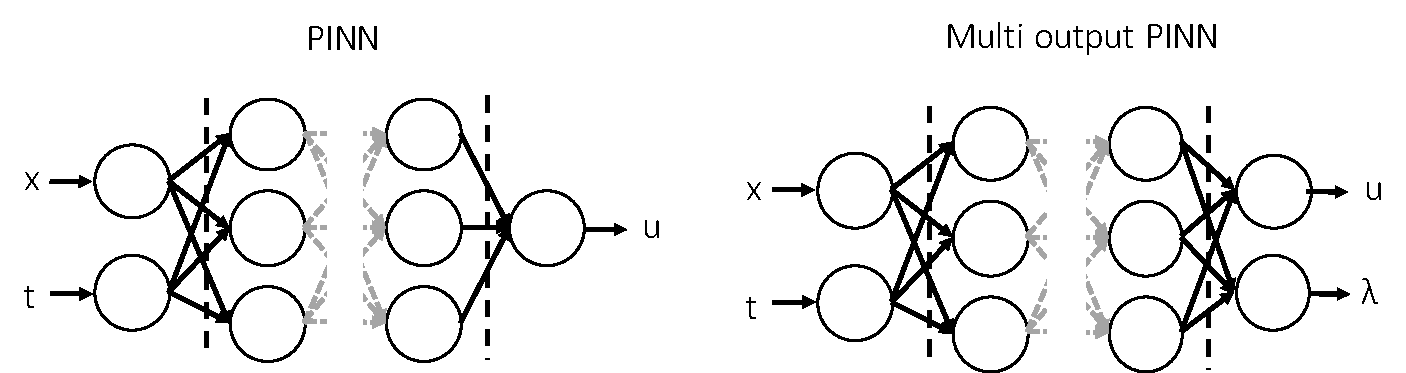
\includegraphics{./tex2pdf.-e2e7a14556ab3e0a/2745f3481242b46bab16e1e6e1123da078cc46ab.pdf}
\caption{Left panel: a normal single output PINN. Right panel: a
multi-output PINN. The network now also predicts the coefficients values
at each data point.}\label{fig:PINN}
}
\end{figure}

\hypertarget{pinns-in-practice}{%
\subsection{PINNs in practice}\label{pinns-in-practice}}

We now wish to evaluate the use of PINNs to analyze the RUSH data. Using
a diffusive process as a toy problem, we first show how PINNs are able
to accurately determine the diffusion constant, even in the presence of
noise. Next, we prove that PINNs are indeed capable of inferring
coefficient fields and finish by analyzing some parts of the RUSH data.

In our toy problem we have an initial concentration profile:

\[
c(x, 0) = e^{-\frac{(x-0.5)^2}{0.02}}
\]

diffusing in a 1D box according to:

\[
\frac{\partial c(x,t)}{\partial t} = \nabla \cdot[D(x)\nabla c(x,t)]
\]

on the spatial domain \([0,1]\) with perfectly absorbing boundaries at
the edges of the domain:

\[
c(0,t) = c(1,t) = 0
\]

If \(D(x) = D\), this problem has an analytical solution through a
Greens function. If the diffusion coefficient is spatially dependent
though, we problem needs to be solved numerically. The code used to
generate our data can be found in the appendix.

\hypertarget{constant-diffusion-coefficient}{%
\subsubsection{Constant diffusion
coefficient}\label{constant-diffusion-coefficient}}

\hypertarget{noiseless}{%
\subsubsection*{Noiseless}\label{noiseless}}
\addcontentsline{toc}{subsubsection}{Noiseless}

Now consider the problem with a constant diffusion of \(D_0 = 0.01\). We
simulate the data on a domain \(x:[0,1]\) and \(t:[0,0.5]\) we use a
spatial resolution of 0.01, giving the number of points 101 by 51,
giving a total number of data points of 5151. Since the fitting is the
training, we do not need to separate the data in a training and
validation set. Figure ref shows the input data and the what the network
predicts. After training, the network predicts (almost exactly) what we
want it to and the average error is less than 1. Ofcourse, more
interesting is the inferred diffusion parameter. With a value of
0.10034, the error is roughly 0.3. This is very good, but ofcourse our
data is without noise. Note however that even still is extremely good
and that in their papers Raissi shows far more complex equations such as
the complex Schrodinger one. Also note that the error is mostly located
at areas with low signal. This is a consistent problem and must be taken
into account. Powerful as they are, neural networks seem to struggle
with this fig.~\ref{fig:Dfield} .

\begin{figure}
\hypertarget{fig:error_constantD}{%
\centering
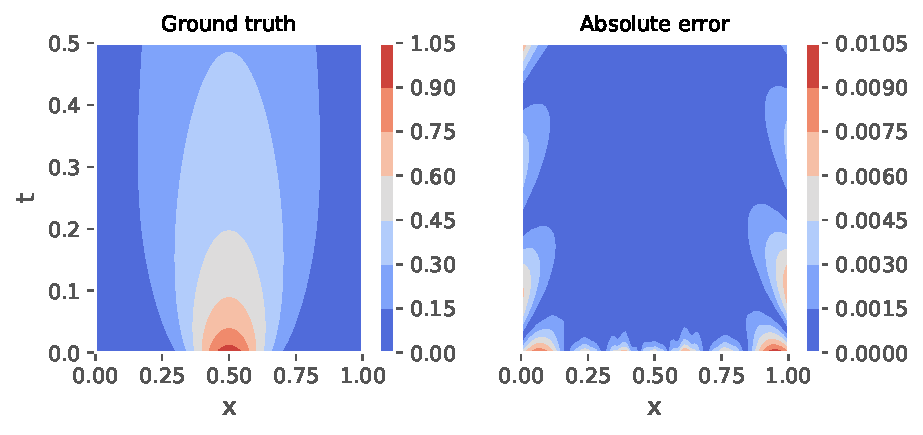
\includegraphics{./tex2pdf.-e2e7a14556ab3e0a/de4bc99c677a83d5cad9eb30f4d895306557c0cb.pdf}
\caption{Left panel: something. Right panel: something
else}\label{fig:error_constantD}
}
\end{figure}

Looks really nice.

\hypertarget{noisy}{%
\subsubsection*{Noisy}\label{noisy}}
\addcontentsline{toc}{subsubsection}{Noisy}

fig.~\ref{fig:Dfield} It becomes more interesting once we add noise. We
take exactly the same problem, but now add 5\% gaussian distributed
white noise (e.g. \(0.05std(c)\)) and let the neural network do it's
thing again. The network is now doing two things at once: it's
\emph{denoising} the data by stating that the underlying data is of a
certain model while finding the optimal model parameters. Again figure
\textbf{ref} shows our original data and the fit.

The data correctly infers the ground truth. The inferred diffusion
coefficient is 0.10017, an error of \(0.17\). I just want to state that
this is almost ridiculous. We have roughly 5000 points with 5 error and
the network is able to infer the coefficent within 1. We also havent
optimized the network in any way: it's the most basic full connected
layers with tanh activation function and we just used enough layers and
neurons. It's also a very general technique: it works for whatever PDE
and data multidimensional data. We also fit the model directly to the
data; circumventing the need to know boundary conditions, initial
conditions etc\ldots{} We can now proceed to more advanced setup.

\begin{figure}
\hypertarget{fig:error_constantD_noisy}{%
\centering
\includegraphics{./tex2pdf.-e2e7a14556ab3e0a/15081e140efb53cca2ad2f9895a54fc385aedc84.pdf}
\caption{Left panel: something. Right panel: something
else}\label{fig:error_constantD_noisy}
}
\end{figure}

\hypertarget{varying-d}{%
\subsubsection{Varying D}\label{varying-d}}

As stated, it should be possible to infer varying coefficient fields.
Instead of using a single output network, we implement of two output
neural network; outputting both the coefficient and the concentration.
Note that this is slightly different from what is done in this paper
\textbf{ref}. They infer the pressure field, but this is a separate
added term; its not multiplied by a spatially varying term.

\hypertarget{non-varying}{%
\subsubsection*{Non-varying}\label{non-varying}}
\addcontentsline{toc}{subsubsection}{Non-varying}

We first demonstrate this using the same data as before: so although we
allow a spatially varying field, the underlying data only has a single
diffusion coefficient. The coefficient is then learned through training
the network and `corrected' by PI-loss function. Figure \textbf{ref}
shows our results.

test reference\textsuperscript{4}

and another one

\hypertarget{varying}{%
\subsubsection*{Varying}\label{varying}}
\addcontentsline{toc}{subsubsection}{Varying}

\hypertarget{real-cell}{%
\subsubsection{Real cell}\label{real-cell}}

\hypertarget{conclusion}{%
\section{Conclusion}\label{conclusion}}

\hypertarget{weak-points-and-how-to-improve}{%
\subsection{Weak points and how to
improve}\label{weak-points-and-how-to-improve}}

\hypertarget{conclusion-1}{%
\chapter{Conclusion}\label{conclusion-1}}

\hypertarget{appendix-1-some-extra-stuff}{%
\chapter*{Appendix 1: Some extra
stuff}\label{appendix-1-some-extra-stuff}}
\addcontentsline{toc}{chapter}{Appendix 1: Some extra stuff}

Add appendix 1 here. Vivamus hendrerit rhoncus interdum. Sed ullamcorper
et augue at porta. Suspendisse facilisis imperdiet urna, eu pellentesque
purus suscipit in. Integer dignissim mattis ex aliquam blandit.
Curabitur lobortis quam varius turpis ultrices egestas.

\footnotesize

\hypertarget{references}{%
\chapter*{References}\label{references}}
\addcontentsline{toc}{chapter}{References}

\hypertarget{refs}{}
\leavevmode\hypertarget{ref-karpatne_physics-guided_2017}{}%
1. Karpatne, A., Watkins, W., Read, J. \& Kumar, V. Physics-guided
Neural Networks (PGNN): An Application in Lake Temperature Modeling.
\emph{arXiv:1710.11431 {[}physics, stat{]}} (2017).

\leavevmode\hypertarget{ref-sharma_weakly-supervised_2018}{}%
2. Sharma, R., Farimani, A. B., Gomes, J., Eastman, P. \& Pande, V.
Weakly-Supervised Deep Learning of Heat Transport via Physics Informed
Loss. \emph{arXiv:1807.11374 {[}cs, stat{]}} (2018).

\leavevmode\hypertarget{ref-pun_physically-informed_2018}{}%
3. Pun, G. P. P., Batra, R., Ramprasad, R. \& Mishin, Y.
Physically-informed artificial neural networks for atomistic modeling of
materials. \emph{arXiv:1808.01696 {[}cond-mat{]}} (2018).

\leavevmode\hypertarget{ref-raissi_physics_2017}{}%
4. Raissi, M., Perdikaris, P. \& Karniadakis, G. E. Physics Informed
Deep Learning (Part II): Data-driven Discovery of Nonlinear Partial
Differential Equations. \emph{arXiv:1711.10566 {[}cs, math, stat{]}}
(2017).

\leavevmode\hypertarget{ref-raissi_physics_2017-1}{}%
5. Raissi, M., Perdikaris, P. \& Karniadakis, G. E. Physics Informed
Deep Learning (Part I): Data-driven Solutions of Nonlinear Partial
Differential Equations. \emph{arXiv:1711.10561 {[}cs, math, stat{]}}
(2017).

\end{document}
